\documentclass[11pt]{article}
\usepackage[margin=1in]{geometry}
\usepackage{amsmath,amssymb,amsthm}
\usepackage{booktabs}
\usepackage{algorithm}
\usepackage{algpseudocode}
\usepackage{longtable}
\usepackage{pgfplots}
\pgfplotsset{compat=1.17}
\usepgfplotslibrary{fillbetween}
\usepackage{hyperref}

\newcommand{\F}{\mathcal{F}}
\newcommand{\E}{\mathbb{E}}
\newcommand{\Var}{\operatorname{Var}}
\newcommand{\lh}{\tilde h}
\newcommand{\lx}{\tilde x}
\newcommand{\unverified}[1]{\textbf{[Not verified against a source: #1]}}
\newcommand{\derived}{\textbf{[Derived here; not stated in the cited papers.]}}

\newtheorem{remark}{Remark}

\title{Realized GARCH, Realized EGARCH and a Likelihood-Based PINN:\\
A Reference for the GARCHPINN Codebase}
\author{Reference document for the rewrite of \texttt{models.py}, \texttt{training.py}, \texttt{data\_utils.py}}
\date{}

\begin{document}
\maketitle

\begin{abstract}
This note fixes the mathematics the code should implement. It states the log-linear
Realized GARCH model of \cite{HHS2012} and the Realized EGARCH model of \cite{HH2016},
shows exactly where the leverage function and the measurement shock enter each, gives the
joint Gaussian quasi-log-likelihood, multi-step forecasts with an exact log-normal-type
bias correction, a physics-informed neural network (PINN) formulation whose loss is the
joint quasi-likelihood, evaluation with QLIKE/MSE \cite{Patton2011} against HAR-RV
\cite{Corsi2009}, and pseudocode. Equations marked \derived{} are my own derivations from the
model equations; anything marked ``Not verified'' could not be checked against a downloaded
source. PDFs are in \texttt{papers/}.
\end{abstract}

\paragraph{Sources used.} Realized GARCH equations are taken from the CREATES working paper
version of \cite{HHS2012} (Research Paper 2010-13, titled ``Realized GARCH: A Complete Model of
Returns and Realized Measures of Volatility''); equation numbering in the published JAE
version may differ, but the model and likelihood are the same.
Realized EGARCH equations are from the published JBES article \cite{HH2016} (author copy).

\tableofcontents

%======================================================================
\section{Notation and data}
%======================================================================

\subsection{Time indices}
Let $t=1,\dots,n$ index \emph{trading days}. Within day $t$ there are $M$ intraday
5-minute intervals with log prices $p_{t,0},p_{t,1},\dots,p_{t,M}$ ($p_{t,0}$ the open,
$p_{t,M}$ the close). Define
\begin{align}
r_{t,j} &= 100\,(p_{t,j}-p_{t,j-1}), \qquad j=1,\dots,M, && \text{(intraday return, \%)} \label{eq:intraday}\\
r^{oc}_t &= 100\,(p_{t,M}-p_{t,0}) = \textstyle\sum_{j=1}^M r_{t,j}, && \text{(open-to-close)} \label{eq:oc}\\
r^{on}_t &= 100\,(p_{t,0}-p_{t-1,M}), && \text{(overnight)} \label{eq:on}\\
r^{cc}_t &= r^{on}_t + r^{oc}_t. && \text{(close-to-close)} \label{eq:cc}
\end{align}
The model is a \textbf{daily} model: $r_t$ is one daily return and $x_t$ one daily realized
measure. The 5-minute data are used only to construct $x_t$. The filtration is
$\F_t=\sigma(r_t,x_t,r_{t-1},x_{t-1},\dots)$ and $h_t=\Var(r_t\mid\F_{t-1})$ \cite{HHS2012}.

\subsection{Realized variance}
The realized variance of day $t$ is the sum of squared intraday returns
\begin{equation}\label{eq:rv}
x_t = RV_t = \sum_{j=1}^{M} r_{t,j}^2 .
\end{equation}
Under a semimartingale price process, $RV_t\to\int_{t-1}^{t}\sigma^2(s)\,ds$ (the integrated
variance of the trading session) as the sampling interval shrinks
\cite{BNS2002,ABDL2003}; \cite{BNS2002} derive its asymptotic distribution.
Sampling at 5 minutes is a conventional compromise against market microstructure noise
\unverified{the specific 5-minute recommendation and noise literature were not downloaded}.

Notes for the implementation:
\begin{itemize}
\item $RV_t$ is a \emph{sum of squares}, not a rolling sample variance. A rolling
  \texttt{var()} demeans and divides by $M-1$; it is not \eqref{eq:rv}.
\item It is computed \emph{once per day} from that day's intervals only (no rolling window
  across days, no overlap).
\item $M$ is the number of 5-minute intervals in the session. For the London Stock
  Exchange continuous session (08:00--16:30 UK time) $M=102$, not the 78 of a 6.5-hour US
  session \unverified{session times should be confirmed against the actual timestamps in
  \texttt{UK\_Index\_2000\_2025.csv}; count intervals per day from the data and drop days
  with many missing bars}.
\item The first interval of a day must start at that day's open; the return from the previous
  close to the first print is the overnight return \eqref{eq:on}, not an intraday return.
\end{itemize}

\subsection{Scaling and units}
Use percentage returns (factor 100) so that daily $h_t$ and $x_t$ are $O(1)$ in \%$^2$;
this keeps $\log h_t,\log x_t$ near zero and makes initial values for $\omega,\xi$ benign.
For 5-minute returns, percent or basis points put $\log h_t$ near $-4.6$ or $+4.6$; the code
scales by $100\sqrt{102}$ (daily-percent-equivalent units) so that $\log h_t\approx0$ again.
Every estimated transform of the 5-minute data (periodicity factor $s_k^2$, zero-range floor)
is computed on training days only, and $s_k$ is indexed by clock time, not bar ordinal.
Do \textbf{not} annualise inside the model. Annualised volatility for reporting only:
$\sigma^{ann}_t = \sqrt{252\,h_t}$ (in \%).

\subsection{The overnight return issue}
$RV_t$ in \eqref{eq:rv} measures only the open-to-close session. Two consistent choices
\cite{HHS2012}:
\begin{enumerate}
\item $r_t=r^{oc}_t$: then $x_t$ and $r_t$ cover the same period, and one expects
  $\varphi\approx1$, $\xi\approx 0$.
\item $r_t=r^{cc}_t$: $h_t$ refers to the full 24 hours while $x_t$ covers only the
  session. HHS explicitly do not impose $\varphi=1$ so that this case is absorbed: $\xi<0$
  (and possibly $\varphi\ne1$) captures the fact that $RV_t$ under-measures daily variance.
\end{enumerate}
HHS report results for both open-to-close and close-to-close returns. Choice 2 is the
default for forecasting daily risk; whichever is used, the evaluation proxy in
Section~\ref{sec:eval} must match the target (e.g.\ compare forecasts of $x_t$ with $RV_t$, or
forecasts of $h_t$ with a proxy that includes the overnight part).

\paragraph{Overnight return in the code \derived.} At 5-min frequency the first bar of day $d$
is kept with its intraday return $\log(\text{Last}/\text{Open})$, and the overnight return
$r^{on}_d$ \eqref{eq:on} is an extra observation at the open, attached to that bar $t$, with
\begin{equation}\label{eq:on-lik}
r^{on}_d\mid\F_{t-1}\sim N\big(0,\;e^{\kappa}h_t\big),\qquad
\ell^{on}_t=-\tfrac12\big[\log2\pi+\kappa+\log h_t+(r^{on}_d)^2e^{-\kappa}/h_t\big],
\end{equation}
added to the return part $\ell_r$ of \eqref{eq:ll-joint} on the rows with an overnight
observation ($\kappa$ is estimated with the other econometric parameters; its ML value given
$h$ is $\log\overline{(r^{on})^2/h_t}$). It does not enter the measurement equation (there is
no intraday range for it), the filter recursion or the network input, and $r^{on}$ is not
divided by the periodicity factor. \texttt{overnight="drop"} (the legacy choice: first bar
dropped, recursion straight across the boundary) remains available; \texttt{"model"} is the 5-min
default. An optional extension, not implemented, is a day-boundary jump in the recursion,
$\log h_{t}\mathrel{+}=\eta_0+\eta_1 z^{on}_d$. Daily stays open-to-close; with
\texttt{daily\_close\_to\_close} the previous close to first-bar close return enters through
\eqref{eq:on-lik} with $h_t$ the daily variance, so $r_t,x_t$ and $\varphi\approx1$ are unchanged.

\paragraph{Bar timestamps.} \texttt{load\_intraday} infers whether stamps mark the bar start or
the bar end (\texttt{bar\_stamp="auto"}) from three votes: the modal first stamp of the day
(session open: start, open $+5$: end), the modal last stamp (session close: start, close
$+5$: end) and which of the bars stamped open or open $+5$ carries the opening-auction $|r|$
($>1.2\times$ the other). The verdict is logged; bar-end stamps are shifted back 5 minutes so
the code always works with bar-start times. \texttt{"start"}/\texttt{"end"} force the convention.

\subsection{Intraday periodicity}
Five-minute absolute returns have a strong deterministic U-shaped intraday pattern which, if
ignored, distorts the estimated dynamics of high-frequency volatility models
\cite{AB1997}. Because the model here runs at the daily frequency and $RV_t$ sums over a
whole session, the periodicity is aggregated out and needs no modelling. \textbf{Running a
GARCH recursion on individual 5-minute returns (as the current code does) is a different
model} and would require a periodic component as in \cite{AB1997}; it is not Realized GARCH.

%======================================================================
\section{Context: GARCH(1,1) and EGARCH}
%======================================================================
With $r_t=\mu+\sqrt{h_t}\,z_t$, $z_t\sim\text{iid}(0,1)$, the GARCH(1,1) model of
\cite{Bollerslev1986} is
\begin{equation}\label{eq:garch}
h_t = \omega + \alpha (r_{t-1}-\mu)^2 + \beta h_{t-1},\qquad \omega>0,\ \alpha,\beta\ge0,\ \alpha+\beta<1 .
\end{equation}
The EGARCH model of \cite{Nelson1991} models the log variance,
\begin{equation}\label{eq:egarch}
\log h_t = \omega + \beta\log h_{t-1} + \theta z_{t-1} + \alpha\bigl(|z_{t-1}|-\E|z_{t-1}|\bigr),
\end{equation}
which needs no positivity constraints and allows asymmetric (leverage) responses. Form
\eqref{eq:egarch} is quoted as written in \cite{HHS2012} (their example of
$\tau(z)=\tau_1 z+\tau_+(|z|-\E|z|)$) and \cite{HH2016} (``$\tau(z)=az+b|z|$'')
\unverified{Nelson (1991) itself was not obtained; his original EGARCH has an ARMA form for
$\log h_t$ and GED innovations}.

These models use only daily returns. Both Realized models below replace the squared-return
ARCH term with a realized measure and add an equation for it.

%======================================================================
\section{Realized GARCH, log-linear form \cite{HHS2012}}
%======================================================================

\subsection{Model}
The log-linear RealGARCH(1,1) model is
\begin{align}
r_t &= \mu + \sqrt{h_t}\, z_t, \label{eq:rg-ret}\\
\log h_t &= \omega + \beta \log h_{t-1} + \gamma \log x_{t-1}, \label{eq:rg-garch}\\
\log x_t &= \xi + \varphi \log h_t + \tau(z_t) + u_t, \label{eq:rg-meas}
\end{align}
with $z_t\sim\text{iid}(0,1)$, $u_t\sim\text{iid}(0,\sigma_u^2)$, $z_t$ and $u_t$ mutually
independent. These are the return, GARCH and measurement equations. HHS write
$r_t=\sqrt{h_t}z_t$; the constant mean $\mu$ is standard and HH2016 note that $\mu=0$ often
forecasts better out of sample.

Key points that the current code gets wrong:
\begin{itemize}
\item In \eqref{eq:rg-garch}, $x_{t-1}$ is the \textbf{observed} realized measure (here
  $RV_{t-1}$). It is not a fitted value. The GARCH equation contains \textbf{no} $\tau$ term
  and no $u$ term.
\item The leverage function $\tau(z_t)$ appears \textbf{only} in the measurement equation
  \eqref{eq:rg-meas}, and with the \emph{contemporaneous} $z_t$. (The code's
  \texttt{delta\_func} is HHS's $\tau$; the code's \texttt{tau\_func} in the GARCH equation
  does not belong in Realized GARCH.)
\item $u_t$ is defined by the measurement equation: $u_t=\log x_t-\xi-\varphi\log
  h_t-\tau(z_t)$.
\end{itemize}

\subsection{Leverage function}
The baseline leverage function is built from Hermite polynomials,
\begin{equation}\label{eq:tau}
\tau(z) = \tau_1 z + \tau_2 (z^2-1),
\end{equation}
so that $\E\tau(z_t)=0$ whenever $\E z_t=0,\ \Var z_t=1$, regardless of the distribution
of $z_t$ \cite{HHS2012}. Higher-order terms $\tau_3(z^3-3z)+\tau_4(z^4-6z^2+3)$ are possible.
Under $z\sim N(0,1)$, $\Var\tau(z)=\tau_1^2+2\tau_2^2$ \derived.

\subsection{Reduced form, stationarity and persistence}
Substituting \eqref{eq:rg-meas} at $t-1$ into \eqref{eq:rg-garch} gives \cite{HHS2012}
\begin{equation}\label{eq:rg-reduced}
\log h_t = \mu_h + \pi \log h_{t-1} + \gamma w_{t-1}, \qquad
\mu_h=\omega+\gamma\xi,\quad \pi=\beta+\varphi\gamma,\quad w_t=\tau(z_t)+u_t ,
\end{equation}
so $\log h_t$ is AR(1) and $\log x_t$ is ARMA(1,1):
\begin{equation}\label{eq:rg-x-arma}
\log x_t = \mu_x + \pi\log x_{t-1} + w_t - \beta w_{t-1}, \qquad \mu_x = \xi(1-\beta)+\varphi\omega .
\end{equation}
($\mu_x$ is \derived; HHS state the ARMA(1,1) form.) The process has a stationary solution if
\begin{equation}\label{eq:rg-stat}
|\pi| = |\beta+\varphi\gamma| < 1 ,
\end{equation}
and $\pi$ is the persistence parameter. Note that $\beta$ alone is \emph{not} the persistence
in Realized GARCH (typical estimates have small $\beta$ and $\pi\approx0.97$--$0.99$).
The stationary mean and variance of $\log h_t$ are
$\E\log h=\mu_h/(1-\pi)$ and $\Var\log h=\gamma^2\sigma_w^2/(1-\pi^2)$,
$\sigma_w^2=\Var\tau(z)+\sigma_u^2$ \derived.
The VARMA form used by HHS for prediction is
\begin{equation}\label{eq:rg-var}
\begin{pmatrix}\lh_t\\ \lx_t\end{pmatrix}
=\begin{pmatrix}\beta&\gamma\\ \varphi\beta&\varphi\gamma\end{pmatrix}
\begin{pmatrix}\lh_{t-1}\\ \lx_{t-1}\end{pmatrix}
+\begin{pmatrix}\omega\\ \xi+\varphi\omega\end{pmatrix}
+\begin{pmatrix}0\\ \tau(z_t)+u_t\end{pmatrix},\qquad \lh_t=\log h_t,\ \lx_t=\log x_t .
\end{equation}

\subsection{Joint Gaussian quasi-log-likelihood}
With Gaussian $z_t$ and $u_t$ the joint density factorises as
$f(r_t,x_t\mid\F_{t-1})=f(r_t\mid\F_{t-1})\,f(x_t\mid r_t,\F_{t-1})$ and \cite{HHS2012}
\begin{equation}\label{eq:ll-joint}
\ell(r,x;\theta) = \underbrace{-\frac12\sum_{t=1}^n\Bigl[\log(2\pi)+\log h_t+\frac{(r_t-\mu)^2}{h_t}\Bigr]}_{\ell(r)\ \text{(partial, returns)}}
\;\underbrace{-\frac12\sum_{t=1}^n\Bigl[\log(2\pi)+\log\sigma_u^2+\frac{u_t^2}{\sigma_u^2}\Bigr]}_{\ell(x\mid r)\ \text{(measurement)}} .
\end{equation}
Here $\theta=(\mu,\omega,\beta,\gamma,\xi,\varphi,\tau_1,\tau_2,\sigma_u^2)$, and $h_t$,
$z_t=(r_t-\mu)/\sqrt{h_t}$, $u_t$ are all functions of $\theta$ via the filter
(Algorithm~\ref{alg:filter}). The likelihood is conditional on $\F_0$, i.e.\ on an initial
value $h_1$. HHS use the density of $\log x_t$ (no Jacobian $-\sum\log x_t$); the Jacobian
does not depend on $\theta$ and can be ignored for estimation but must be kept consistent
when comparing with models for $x_t$ in levels.

The partial likelihood $\ell(r)$ is comparable with the likelihood of a standard GARCH model;
the joint $\ell(r,x)$ is not \cite{HHS2012}. Concentrating out $\sigma_u^2$,
$\hat\sigma_u^2(\theta)=n^{-1}\sum_t u_t^2$, gives
\begin{equation}\label{eq:ll-conc}
\ell^c(\theta) = -\frac12\sum_{t=1}^n\Bigl[\log h_t + z_t^2\Bigr] - \frac n2\log\hat\sigma_u^2(\theta) + \text{const},
\end{equation}
which is the scalar version of the concentrated likelihood in \cite{HH2016}. QMLE is
consistent under misspecification of the Gaussian shape; HHS give analytic scores and Hessians.

\textbf{The training loss of the rewritten code is $-\ell(r,x;\theta)/n$} (or
$-\ell^c/n$), not a sum of MSEs. A sum of MSEs gives equal weight to returns in levels and
to log-RV residuals, ignores $\log h_t$ (the term that stops $h_t\to\infty$), and is not a
likelihood for any model.

%======================================================================
\section{Realized EGARCH \cite{HH2016}}
%======================================================================
With $K$ realized measures $x_{k,t}$ ($K=1$ here),
\begin{align}
r_t &= \mu_t + \sqrt{h_t}\,z_t, \label{eq:reg-ret}\\
\log h_t &= \omega + \beta\log h_{t-1} + \tau(z_{t-1}) + \gamma' u_{t-1}, \label{eq:reg-garch}\\
\log x_{k,t} &= \xi_k + \varphi_k \log h_t + \delta^{(k)}(z_t) + u_{k,t}, \label{eq:reg-meas}
\end{align}
$z_t\sim N(0,1)$, $u_t\sim N(0,\Sigma_u)$ independent, and
$\tau(z)=\tau_1 z+\tau_2(z^2-1)$, $\delta^{(k)}(z)=\delta_{k,1}z+\delta_{k,2}(z^2-1)$.
The volatility shock is $v_t=\E(\log h_{t+1}\mid\F_t)-\E(\log h_{t+1}\mid\F_{t-1})=\tau(z_t)+\gamma'u_t$.
The GARCH equation is an AR(1) in $\log h_t$ with innovation $\tau(z_{t-1})+\gamma'u_{t-1}$,
so $\beta$ \emph{is} the persistence; stationarity requires $|\beta|<1$. HH2016 stress that
the Realized GARCH of \cite{HHS2012} ``only includes a leverage function in the measurement
equation''. The concentrated quasi-likelihood is
$\ell\propto-\frac12\sum_t[\log h_t+z_t^2]-\frac n2\log|\hat\Sigma_u|$, same structure as
\eqref{eq:ll-conc}.

\begin{table}[h]
\centering\small
\caption{Realized GARCH vs.\ Realized EGARCH ($K=1$). The current code is a hybrid of the two
columns, which is neither model.}
\label{tab:compare}
\begin{tabular}{@{}lll@{}}
\toprule
& Realized GARCH (log-linear) \cite{HHS2012} & Realized EGARCH \cite{HH2016}\\
\midrule
GARCH eq.\ driver & $\gamma\log x_{t-1}$ (observed RV) & $\gamma u_{t-1}$ (measurement shock)\\
$\tau(z)$ in GARCH eq. & no & yes, $\tau(z_{t-1})$\\
leverage in measurement eq. & $\tau(z_t)$ & $\delta(z_t)$ (second function)\\
number of leverage functions & 1 & 2\\
persistence & $\pi=\beta+\varphi\gamma$ & $\beta$\\
stationarity & $|\beta+\varphi\gamma|<1$ & $|\beta|<1$\\
needs $u_{t-1}$ for $h_t$ & no (only $x_{t-1}$) & yes\\
multiple $x$'s & possible & natural ($\gamma$ vector, $\Sigma_u$)\\
\midrule
\textbf{current code} & \multicolumn{2}{l}{$\log h_t=\omega+\beta\log h_{t-1}+\tau(z_{t-1})+\gamma\,\widehat{\log x}_{t-1}$, measurement with $\delta(z_t)$}\\
\bottomrule
\end{tabular}
\end{table}

The two models are closely related: substituting \eqref{eq:rg-meas} into
\eqref{eq:rg-garch} gives $\log h_t=\mu_h+\pi\log h_{t-1}+\gamma\tau(z_{t-1})+\gamma u_{t-1}$,
which is a Realized EGARCH with GARCH-equation leverage $\gamma\tau(\cdot)$ and
$\gamma_{\text{REG}}=\gamma$ \derived. Using the \emph{fitted} $\widehat{\log x}_{t-1}=\xi+\varphi\log h_{t-1}+\delta(z_{t-1})$
instead of the observed $\log x_{t-1}$, as the code does, deletes $u_{t-1}$ from the recursion,
so the realized measure never feeds back into $h_t$ and the model collapses to an EGARCH
on returns alone.

\paragraph{Decision for the rewrite.} Implement Realized GARCH \eqref{eq:rg-ret}--\eqref{eq:rg-meas}
as the primary model (the code is named after it). Optionally implement Realized EGARCH as a
separate class with its own \texttt{tau}/\texttt{delta}; never mix the two.

%======================================================================
\section{Multi-step forecasting}\label{sec:forecast}
%======================================================================
At the end of day $t$, $h_{t+1}$ is known exactly from \eqref{eq:rg-garch}:
$\log h_{t+1}=\omega+\beta\log h_t+\gamma\log x_t$, using the observed $x_t$.
For $k\ge2$, iterate \eqref{eq:rg-reduced}; future $z,u$ are unknown, and since
$\E\tau(z)=0$ and $\E u=0$ the shocks drop out of the conditional mean:
\begin{equation}\label{eq:fc-logh}
\E_t[\log h_{t+k}] = \mu_h\sum_{j=0}^{k-2}\pi^j + \pi^{k-1}\log h_{t+1},\qquad k\ge1 .
\end{equation}
\derived{} (direct consequence of \eqref{eq:rg-reduced}; HHS give the equivalent VARMA
iteration of \eqref{eq:rg-var}.)

\textbf{Pitfall in the current \texttt{forecast\_volatility}:} it sets $z,u$ to zero
\emph{inside} $\tau(z)=\tau_1z+\tau_2(z^2-1)$, which gives $\tau(0)=-\tau_2\neq0$; the correct
conditional expectation uses $\E\tau(z)=0$, i.e.\ drop the $\tau$ term. It also uses the
Realized EGARCH form ($\gamma u$) with Realized GARCH parameters, and iterates with
$\beta$ instead of $\pi$.

\paragraph{Bias (Jensen) correction for $h$.} $\E_t[h_{t+k}]\neq\exp\E_t[\log h_{t+k}]$. Write
$\log h_{t+k}=\E_t\log h_{t+k}+\gamma\sum_{j=0}^{k-2}\pi^j w_{t+k-1-j}$ with $w$ iid. With
$z\sim N(0,1)$ and $u\sim N(0,\sigma_u^2)$ independent, for $c$ with $1-2c\tau_2>0$,
\begin{equation}\label{eq:mgf}
\Psi(c):=\E e^{c\,w}=\E e^{c\tau(z)}\,\E e^{cu}
=\frac{1}{\sqrt{1-2c\tau_2}}\exp\Bigl(-c\tau_2+\frac{c^2\tau_1^2}{2(1-2c\tau_2)}+\frac{c^2\sigma_u^2}{2}\Bigr),
\end{equation}
so that, exactly under Gaussianity, \derived
\begin{equation}\label{eq:fc-h}
\E_t[h_{t+k}] = \exp\bigl(\E_t\log h_{t+k}\bigr)\prod_{j=0}^{k-2}\Psi(\gamma\pi^j) .
\end{equation}
The second-order approximation is $\E_t h_{t+k}\approx\exp\bigl(\E_t\log h_{t+k}+\tfrac12 V_k\bigr)$,
$V_k=\gamma^2\sigma_w^2\sum_{j=0}^{k-2}\pi^{2j}$. If $z$ is not Gaussian, use the empirical
average of $e^{c\hat w_t}$ over in-sample residuals (non-parametric, also \derived), or simulate
with Algorithm~\ref{alg:sim} using bootstrapped $(\hat z_t,\hat u_t)$.
In the code the empirical MGF is the default for 5-min data (\texttt{forecast\_mgf}), since a large
estimated $\tau_2$ (or $\delta_2$) makes the Gaussian $\Psi$ badly biased there; the Gaussian
forecasts are still reported (\texttt{*\_gauss}). Daily stays Gaussian, with \texttt{*\_emp} alongside.

\paragraph{Forecasting the realized measure.} From \eqref{eq:rg-meas},
$\E_t\log x_{t+k}=\xi+\varphi\E_t\log h_{t+k}$ and, in levels \derived,
\begin{equation}\label{eq:fc-x}
\E_t[x_{t+k}] = e^{\xi}\,e^{\varphi\E_t\log h_{t+k}}\,\Psi_\tau(1)\,e^{\sigma_u^2/2}\,
\prod_{j=0}^{k-2}\Psi(\varphi\gamma\pi^j),
\end{equation}
where $\Psi_\tau(1)=\E e^{\tau(z)}=(1-2\tau_2)^{-1/2}\exp(-\tau_2+\tau_1^2/(2(1-2\tau_2)))$
(contemporaneous $z_{t+k}$ and $u_{t+k}$ are independent of $h_{t+k}$). Use \eqref{eq:fc-x}
when evaluating against $RV_{t+k}$, and \eqref{eq:fc-h} against a close-to-close proxy.

For Realized EGARCH: $\E_t\log h_{t+k}=\omega\sum_{j=0}^{k-2}\beta^j+\beta^{k-1}\log h_{t+1}$,
with the analogous correction using $w=\tau(z)+\gamma u$ and $c=\beta^j$ \derived.
For $k=1$ the products are empty, so only $1-2\delta_2>0$ (measurement term) is required.

\paragraph{With the NN correction.} The closed form is exact only for $g\equiv0$. The known
$g_t$ is inside $\log h_{t+1}$; for $k\ge2$ one must use $\E_t g_{t+j}$, not a frozen $g_t$
(freezing adds $g_t(1-\pi^{k-1})/(1-\pi)$ to $\E_t\log h_{t+k}$). The code uses the training
mean $\bar g$ for steps $\ge2$ (approximate) and offers Monte Carlo in which the HAR features
are recomputed from simulated $\log x$ and the calendar is advanced deterministically.
Gaussian $\Psi$ is replaced, optionally, by the empirical mean of $e^{c\hat w_t}$ and of
$e^{\delta(\hat z_t)+\hat u_t}$ over training residuals; both variants are reported.

%======================================================================
\section{Parameter constraints and reparameterisations}\label{sec:param}
%======================================================================
Train unconstrained raw parameters and map them:
\begin{center}
\begin{tabular}{@{}lll@{}}
\toprule
Parameter & Constraint & Map from raw $a\in\mathbb R$\\
\midrule
$\pi=\beta+\varphi\gamma$ & $|\pi|<1$ (in practice $0<\pi<1$) & $\pi = 0.9999\,\sigma(a_\pi)$\\
$\gamma$ & $\ge0$ (empirically) & $\gamma=\operatorname{softplus}(a_\gamma)$ or free\\
$\varphi$ & $>0$ & $\varphi=\exp(a_\varphi)$ or free\\
$\beta$ & implied & $\beta=\pi-\varphi\gamma$\\
$\sigma_u^2$ & $>0$ & $\sigma_u^2=\exp(a_u)$ (or concentrate out, \eqref{eq:ll-conc})\\
$\tau_2$ & $1-2c\tau_2>0$ for \eqref{eq:mgf} & usually small; check post-fit\\
$\omega,\xi,\mu,\tau_1$ & none & identity\\
$\log h_1$ & --- & free parameter (as in \cite{HH2016}) or $\log$ of sample var of $r$ over a burn-in\\
\bottomrule
\end{tabular}
\end{center}
Parameterising by $\pi$ enforces \eqref{eq:rg-stat} exactly; $\beta$ itself may be negative
and must not be clamped to $(0,1)$. The reparameterisation is a modelling choice
\derived. Initial values close to typical estimates (e.g.\ $\pi\approx0.97$,
$\gamma\approx0.4$, $\varphi\approx1$, $\tau_1\approx-0.07$, $\tau_2\approx0.07$,
$\sigma_u\approx0.4$; magnitudes as in the SPY/DJIA tables of \cite{HHS2012}
\unverified{exact table values not transcribed}) speed up convergence. Use float64; avoid
\texttt{clamp} inside the recursion (zero gradients). \textbf{Correction:} a soft bound
$B\tanh(\log h_t/B)$ is \emph{not} acceptable: $B\tanh(y/B)=y-y^3/(3B^2)+\dots$ has slope
$\operatorname{sech}^2(y/B)$, so it multiplies the effective persistence by $\approx1-y^2/B^2$
(0.93 at $y=4$, $B=15$) and shifts the fixed point; QMLE then pushes $\pi$ to its cap and the
closed-form forecasts \eqref{eq:fc-h} no longer describe the filter \derived. Any guard must be
the identity on the reachable range, e.g.\ with $c$ the (detached) training log variance and
$d=\log h-c$: $c+d-\operatorname{softplus}(d-B)+\operatorname{softplus}(-d-B)$, whose deviation from the
identity is $O(e^{-(B-|d|)})$; and returns should be scaled so that $\log h_t\approx0$.

\textbf{Filter stability.} $|\pi|<1$ gives a stationary DGP but not a stable filter. For
Realized GARCH, $\partial\log h_t/\partial\log h_{t-1}$ given observed $x$ is $\beta$, so also
$|\beta|<1$ is needed (HHS Lemma~1). For Realized EGARCH the condition is
$\E\log|A(z_t)|<0$, $A(z)=\beta-\gamma\varphi-\tfrac z2(\tau_1-\gamma\delta_1)-z^2(\tau_2-\gamma\delta_2)$
(\cite{HH2016}, eq.~3; own derivative). Both are reported post-fit.

%======================================================================
\section{A PINN formulation}\label{sec:pinn}
%======================================================================

\subsection{Where the neural network enters}
The ``physics'' is the Realized GARCH law of motion. The network $g_\eta$ is an additive
correction to the GARCH equation that must be $\F_{t-1}$-measurable:
\begin{equation}\label{eq:pinn-garch}
\log h_t = \omega + \beta\log h_{t-1} + \gamma\log x_{t-1} + s\,g_\eta(\mathbf{f}_{t-1}),
\qquad \mathbf f_{t-1}=\bigl(\log x_{t-1},\overline{\log x}^{(w)}_{t-1},\overline{\log x}^{(m)}_{t-1}, z_{t-1}, \log h_{t-1}, \text{calendar}_t\bigr),
\end{equation}
with the return and measurement equations \eqref{eq:rg-ret}, \eqref{eq:rg-meas} unchanged.
$\overline{\log x}^{(w)},\overline{\log x}^{(m)}$ are 5- and 22-day averages, the HAR
components of \cite{Corsi2009}, which capture long memory that a single AR(1) misses.
Inputs must not include $z_t$, $u_t$ or $x_t$ (look-ahead): $h_t$ is by definition
$\F_{t-1}$-measurable \cite{HHS2012}. A scale $s$ (learned, initialised near 0) or zero-init
of the last layer makes the model start exactly at Realized GARCH. This design follows the
hybrid literature in which a recurrent network augments the Realized GARCH recursion and the
whole model is fitted by likelihood \cite{Liu2023}; see also \cite{Xu2024,Zhao2024}.
No BatchNorm inside a time recursion (batch statistics mix time steps and windows); use
LayerNorm or none.

\subsection{Loss}
\begin{equation}\label{eq:pinn-loss}
\mathcal L(\theta,\eta) = -\frac1n\,\ell(r,x;\theta,\eta)
\;+\;\lambda_{\text{m}}\,\mathcal R_{\text{moment}}
\;+\;\lambda_g\,\frac1n\sum_t g_\eta(\mathbf f_{t-1})^2
\;+\;\lambda_w\|\eta\|^2 ,
\end{equation}
with $\ell$ from \eqref{eq:ll-joint} computed from the filtered $h_t$ of \eqref{eq:pinn-garch}.
The likelihood is the data-fit term; there is no separate ``data loss'' on $\exp(\widehat{\log x})$.

\paragraph{Orthogonality penalty.} The code adds $\lambda_{\rm orth}P_{\rm orth}$ with
\begin{equation}\label{eq:pinn-orth}
P_{\rm orth}=\bar g^2+\sum_{k}\widehat{\operatorname{cov}}\big(g_t,\;q_{k,t-1}/\widehat{\rm sd}(q_k)\big)^2,
\end{equation}
where $q_{k,t-1}$ (detached) are the non-constant regressors of the GARCH equation:
$\log h_{t-1},\log x_{t-1}$ for Realized GARCH and $\log h_{t-1},z_{t-1},z_{t-1}^2-1,u_{t-1}$ for
Realized EGARCH. Without the $\log x_{t-1}$ (resp.\ $z,u$) terms $g$ could absorb part of $\gamma$
(resp.\ $\tau_1,\tau_2,\gamma$), so $g$ is identified only as the component orthogonal to all of them.
\paragraph{Stage-2 schedule.} The econometric parameters start at the QMLE; Adam's steps of size
$\approx$\,lr per coordinate would move them before $g$ has learned anything. They are therefore
frozen for the first \texttt{econ\_warmup} epochs, then trained with lr$\times$\texttt{econ\_lr\_mult};
both groups follow a cosine decay and early-stopping patience counts only after the warm-up.

\paragraph{Computation at 5-min.} Only $\log h_t$ is on the sequential path. The filter rewrites
the GARCH equation with $u_t$ substituted from the measurement equation,
$\log h_{t+1}=a_t+b\log h_t+k_z z_t+k_e(z_t^2-1)+s\,g_t$ with $a_t=\omega+\gamma\log x_t$, $b=\beta$, $k_z=k_e=0$ (GARCH) or
$a_t=\omega-\gamma\xi+\gamma\log x_t$, $b=\beta-\gamma\varphi$, $k_z=\tau_1-\gamma\delta_1$,
$k_e=\tau_2-\gamma\delta_2$ (EGARCH; exact algebra), precomputes $a_t$, the exo part of the first network
layer (or all of $g_t$ when the network does not read the state), and recovers $z_t,u_t$ after
the loop in one vectorised pass; without autograd the loop runs in numpy. Results agree with
the step-by-step filter to $10^{-15}$. Since the cost is the number of sequential steps,
the 5-min defaults use 256 stage-1 and 128 stage-2 streams (each with the 102-bar burn-in
masked, about 6\% and 3\% of the 455k training bars of 650k), at most 150 L-BFGS iterations, 30 epochs, warm-up 5 and
patience 8.

\subsection{Physics residuals that are not identically zero}
The model implies population moment conditions that hold only at the true parameters and
true $h_t$ (from the iid/independence assumptions of \cite{HHS2012} and the conditions
$\E(u_t\mid z_t,\F_{t-1})=0$, $\E(u_t^2\mid\F_{t-1})=\sigma_u^2$ in \cite{HH2016}):
\begin{equation}\label{eq:moments}
\begin{aligned}
&\E z_t=0, \quad \E(z_t^2-1)=0, \quad \E u_t=0,\quad \E[u_t z_t]=0,\quad \E[u_t(z_t^2-1)]=0,\\
&\E[(z_t^2-1)(z_{t-\ell}^2-1)]=0,\quad \E[u_tu_{t-\ell}]=0,\quad \E[u_t z_{t-\ell}]=0,\qquad \ell=1,\dots,L .
\end{aligned}
\end{equation}
Let $\bar m$ be the vector of sample averages of these products over the $n$ unmasked
observations of a TBPTT chunk and $\widehat{\rm se}_j^2=\overline{m_j^2}/n$ (detached). The
code uses the standardised (diagonal-GMM) form
$\mathcal R_{\text{moment}}=\frac1n\sum_j \bar m_j^2/\widehat{\rm se}_j^2$ (\texttt{moment\_standardize});
under correct specification it is about $\chi^2_k/n$. The raw $\|\bar m\|^2$ has a noise floor
$\sum_j\operatorname{var}(m_j)/n\approx0.1$--$0.2$ per chunk (from $\operatorname{var}[(z_t^2-1)(z_{t-\ell}^2-1)]\approx4$),
comparable to the whole likelihood gain of $g$, and its gradient moved the econometric parameters
off the QMLE, so stage 2 never improved the validation NLL.
These are genuine constraints: a network that overfits the conditional mean of $\log x$ or
lets $h_t$ chase $r_t^2$ leaves autocorrelation in $z_t^2$ or $u_t$. They are a weighted
GMM-type penalty and \textbf{are a design proposal} \derived; several of them are already
first-order conditions of \eqref{eq:ll-joint} at the QMLE (e.g.\ the $\xi$-score gives
$\sum u_t=0$), so they matter mostly for $\eta$ and at lags $\ell\ge1$.
An additional optional residual is the reduced-form check: with $\hat w_t=\tau(\hat z_t)+\hat u_t$,
$\rho_t=\log h_t-\mu_h-\pi\log h_{t-1}-\gamma\hat w_{t-1}-s g_\eta(\mathbf f_{t-1})$ is zero
by algebra and is only a unit test, \emph{not} a loss term.

\subsection{Related design: GARCH-informed neural networks (GINN) \cite{Xu2024}}
Xu et al.\ fit daily close-to-close returns $r_t=\mu_t+\varepsilon_t$, $\varepsilon_t=\sigma_t e_t$,
$e_t\sim N(0,1)$. A rolling AR model on the last 90 returns gives $\hat\mu_t$, and the variance
``ground truth'' is the squared residual $\sigma^2_t:=(r_t-\hat\mu_t)^2$. A rolling constant-mean
GARCH(1,1), $\sigma_t^2=\alpha_0+\alpha\varepsilon_{t-1}^2+\beta\sigma_{t-1}^2$, re-fitted on each
90-day window (Python \texttt{arch}), gives $\hat\sigma^2_{t,\mathrm{GARCH}}$. The network is
$\hat\sigma^2_{t,\mathrm{GINN}}=\mathrm{LSTM}(\sigma^2_{t-90},\dots,\sigma^2_{t-1})$: three LSTM layers of width
256 with dropout, two linear layers, one BatchNorm and a ReLU output, trained with AdamW for about 300
epochs. The loss is
\begin{equation}\label{eq:ginn-loss}
\mathcal L_{\mathrm{GINN}}=\lambda\,\mathrm{MSE}\bigl(\sigma^2_t,\hat\sigma^2_{t,\mathrm{GINN}}\bigr)
+(1-\lambda)\,\mathrm{MSE}\bigl(\hat\sigma^2_{t,\mathrm{GARCH}},\hat\sigma^2_{t,\mathrm{GINN}}\bigr),
\end{equation}
with $\lambda$ chosen by grid search ($0$ to $1$) on a separate index (NASDAQ), giving $\lambda=0.01$.
GINN-0 ($\lambda=0$) distils GARCH only and performs about as well. Evaluation uses
$R^2$, MSE and MAE against $(r_t-\hat\mu_t)^2$ on a 70/30 chronological split of 7 indices,
FTSE 100 among them.

\emph{Relation to this document.} Here GARCH is a soft teacher, not a structural law of motion. The
NN output is not fed back into any recursion, there is no realized measure, no measurement equation
and no likelihood. The loss is MSE on variances, which is dominated by extreme days. Its
``physics'' term is therefore a distillation penalty, not a residual of \eqref{eq:pinn-garch}. We do
not adopt \eqref{eq:ginn-loss}. The likelihood \eqref{eq:ll-joint} already contains the GARCH
structure exactly. The analogue of its regularisation toward GARCH is the penalty $\lambda_g\sum g_\eta^2$
in \eqref{eq:pinn-loss}, together with the zero-initialised correction. Two lessons carry over:
(i) the authors' best result is nearly pure GARCH ($\lambda\approx0$), so the NN correction should
start at, and be shrunk toward, the econometric model; and (ii) $\lambda$ should be tuned on held-out
validation data, never on the test set. Its use of BatchNorm and of $r_t^2$ as the target conflicts with
the Pitfalls below and with \S\ref{sec:eval} (QLIKE with realized proxies \cite{Patton2011}).

\subsection{Pitfalls (each present in the current code)}
\begin{enumerate}
\item \textbf{Identically-zero residuals.} If $z_t$ is defined as $(r_t-\mu)/\sqrt{h_t}$ then
  $r_t-\mu-\sqrt{h_t}z_t\equiv0$; if $h_t$ is produced by the GARCH recursion then the
  ``GARCH residual'' $\log h_t-(\omega+\dots)\equiv0$ (up to clamps and the NN term). Such
  terms carry no information; their only effect is to penalise the NN correction through
  the back door and to waste gradient. Remove them.
\item \textbf{Circular use of fitted $\log x$.} The GARCH equation must use the observed
  $\log x_{t-1}$. Using $\widehat{\log x}_{t-1}$ removes the information in the realized
  measure (Table~\ref{tab:compare}).
\item \textbf{Measurement fit against a fitted value that already contains $\tau(z_t)$
  computed from $r_t$}: fine inside the likelihood (that is the model), but an extra MSE on
  $\exp(\widehat{\log x}_t)-x_t$ double-counts the measurement density in the wrong scale.
\item \textbf{Look-ahead in the NN}: feeding $z_t,u_t$ into a correction of $\log h_t$.
\item \textbf{Smoothness penalty on $\log h_t$}: there is no such term in the model; the
  dynamics are already governed by $\pi$. Remove.
\item \textbf{Short shuffled windows with re-initialised $h$}: re-starting the filter at
  every 20-step window from $\log x$ of the window's first step biases $h$ and discards the
  long memory ($\pi\approx0.98$ has half-life $\approx35$ days). Run the filter over the full
  training sample (or long contiguous chunks with carried-over state; truncated BPTT).
\item \textbf{Clamps} on $z,\log h,\log x,u$ zero the gradient whenever active, and clamping
  squared errors at 100 caps the likelihood. Remove or replace with smooth bounds.
\end{enumerate}

%======================================================================
\section{Evaluation}\label{sec:eval}
%======================================================================
\subsection{Loss functions}
For a variance forecast $h$ and a conditionally unbiased proxy $\hat\sigma^2$
(here $RV_{t+k}$, matching the target as discussed in Section~1), \cite{Patton2011} gives
\begin{align}
\text{MSE}:\quad & L(\hat\sigma^2,h) = (\hat\sigma^2-h)^2, \label{eq:mse}\\
\text{QLIKE}:\quad & L(\hat\sigma^2,h) = \log h + \hat\sigma^2/h . \label{eq:qlike}
\end{align}
MSE and QLIKE are the only common losses that rank forecasts consistently when the proxy is
noisy (``robust''); QLIKE depends only on $\hat\sigma^2/h$ and is less sensitive to extreme
observations, whereas MSE-on-logs and MSE on standard deviations are not robust
\cite{Patton2011}. The normalised variant $\hat\sigma^2/h-\log(\hat\sigma^2/h)-1\ge0$ ranks
identically \unverified{this normalisation is standard but was not located in the downloaded
version}. Do \textbf{not} evaluate with MSE on $\log$ RV only. Report losses on daily, not
annualised, units.

\subsection{Out-of-sample protocol}
\begin{enumerate}
\item Split by date, never by shuffled windows: e.g.\ estimation 2000--2014, validation
  2015--2017 (choose $\lambda$'s, network size, early stopping on validation $-\ell$),
  test 2018--end.
\item Rolling or expanding window: re-estimate every $R$ days (e.g.\ 21 or 63); between
  re-estimations run the filter forward with fixed parameters using observed $(r_t,x_t)$.
\item Forecast horizons $k=1,5,22$ with \eqref{eq:fc-h}/\eqref{eq:fc-x}; for multi-day
  targets compare $\sum_{i=1}^k\E_t x_{t+i}$ with $\sum_{i=1}^k RV_{t+i}$.
\item Report average out-of-sample QLIKE and MSE, the out-of-sample partial log-likelihood
  $\ell(r)$ (as HHS do), and test differences with a Diebold--Mariano test
  \unverified{DM and Model Confidence Set papers not downloaded}. For overlapping $k$-step
  targets the loss differential is at least MA$(k-1)$; a Bartlett kernel truncated at $k-1$
  underestimates its long-run variance by about one third \derived. Use a data-driven
  bandwidth (Newey--West 1994) with a floor of $2(k-1)$, the Harvey--Leybourne--Newbold factor
  and $t_{n-1}$ critical values. GARCH(1,1) forecasts $\E h$, not $\E x$: score it after a
  proxy map $\hat c=\overline{x}/\overline{h}$ estimated on the training split, since QLIKE
  of a perfect forecast scaled by $c\neq1$ is $c-\log c-1>0$ \cite{Patton2011}. Fit all
  models on the same estimation window.
\item Benchmarks: GARCH(1,1) \eqref{eq:garch}, plain Realized GARCH (the PINN with $g\equiv0$),
  and HAR-RV.
\end{enumerate}

\subsection{HAR-RV benchmark}
\cite{Corsi2009}:
\begin{equation}\label{eq:har}
RV_{t+1} = c + \beta^{(d)}RV_t + \beta^{(w)}RV^{(w)}_t + \beta^{(m)}RV^{(m)}_t + \omega_{t+1},\quad
RV^{(w)}_t=\tfrac15\sum_{i=0}^{4}RV_{t-i},\quad RV^{(m)}_t=\tfrac1{22}\sum_{i=0}^{21}RV_{t-i},
\end{equation}
estimated by OLS (with HAC standard errors). Corsi writes the model for realized volatility
(the square root); the same regression on $RV$ in variance units or on $\log RV$ is common.
For a log-HAR, the level forecast needs a bias correction $\exp(\widehat{\log RV}+\hat s^2/2)$
\derived. $k$-step forecasts: direct regression of $\frac1k\sum_{i=1}^k RV_{t+i}$ on the same
regressors.

%======================================================================
\section{Algorithms}
%======================================================================

\begin{algorithm}[h]
\caption{Realized GARCH filter (log-linear, with optional NN correction)}\label{alg:filter}
\begin{algorithmic}[1]
\Require returns $r_{1:n}$, observed realized measures $x_{1:n}>0$, parameters $\theta$, initial $\lh_1$, network $g_\eta$ (or $g\equiv0$)
\State $\ell_r\gets0$, $\ell_x\gets0$
\For{$t=1$ to $n$}
  \If{$t>1$}
    \State $\lh_t\gets\omega+\beta\lh_{t-1}+\gamma\log x_{t-1}+s\,g_\eta(\mathbf f_{t-1})$ \Comment{observed $x_{t-1}$; no $\tau$ here}
  \EndIf
  \State $z_t\gets(r_t-\mu)\,e^{-\lh_t/2}$
  \State $u_t\gets\log x_t-\xi-\varphi\lh_t-\tau_1z_t-\tau_2(z_t^2-1)$
  \State $\ell_r\gets\ell_r-\frac12[\log2\pi+\lh_t+z_t^2]$
  \State $\ell_x\gets\ell_x-\frac12[\log2\pi+\log\sigma_u^2+u_t^2/\sigma_u^2]$
\EndFor
\State $\lh_{n+1}\gets\omega+\beta\lh_n+\gamma\log x_n+s\,g_\eta(\mathbf f_n)$ \Comment{one-step forecast}
\State \Return $\lh_{1:n+1}$, $z_{1:n}$, $u_{1:n}$, $\ell_r$, $\ell_x$
\end{algorithmic}
\end{algorithm}

\begin{algorithm}[h]
\caption{QMLE / gradient training of the PINN}\label{alg:train}
\begin{algorithmic}[1]
\Require training sample $(r_t,x_t)_{t=1}^{n}$, validation sample, raw parameters $a$ (Section~\ref{sec:param}), $\eta$
\State \textbf{Stage 1 (pure Realized GARCH):} set $g\equiv0$; maximise $\ell$ over $\theta$ with L-BFGS on the full sequence (float64); this is the QMLE benchmark
\State \textbf{Stage 2 (PINN):} initialise $\theta$ at Stage-1 estimate, last NN layer $=0$
\For{epoch $=1,\dots,E$}
  \State split the training sequence into $B$ contiguous chunks; carry $\lh$ across chunk boundaries (detached for truncated BPTT)
  \For{each chunk in time order}
    \State map raw $a\mapsto\theta$; run Algorithm~\ref{alg:filter} on the chunk
    \State compute $\mathcal L$ in \eqref{eq:pinn-loss} (likelihood + moment residuals \eqref{eq:moments} + penalties)
    \State $\nabla_{a,\eta}\mathcal L$ by autodiff; clip gradient norm; Adam step
  \EndFor
  \State run filter on validation sample (state carried from end of training); record $-\ell_{\text{val}}$ and QLIKE
  \If{no validation improvement for $P$ epochs} \textbf{stop}, restore best \EndIf
\EndFor
\State \Return $\hat\theta,\hat\eta$; report $\hat\pi$, $\hat\sigma_u$, $\ell(r)$, $\ell(r,x)$
\end{algorithmic}
\end{algorithm}

\begin{algorithm}[h]
\caption{$k$-step forecasting (pure Realized GARCH; with NN, use simulation, Algorithm~\ref{alg:sim})}\label{alg:fc}
\begin{algorithmic}[1]
\Require $\hat\theta$, $\lh_{t+1}$ from the filter (uses observed $x_t$), horizon $K$
\State $m_1\gets\lh_{t+1}$, $C_1\gets1$
\For{$k=2$ to $K$}
  \State $m_k\gets\mu_h+\pi m_{k-1}$ \Comment{$\mu_h=\omega+\gamma\xi$, $\pi=\beta+\varphi\gamma$; $\E\tau(z)=\E u=0$}
  \State $C_k\gets C_{k-1}\cdot\Psi(\gamma\pi^{k-2})$ \Comment{\eqref{eq:mgf}}
\EndFor
\For{$k=1$ to $K$}
  \State $\E_t\log h_{t+k}\gets m_k$;\quad $\E_t h_{t+k}\gets e^{m_k}C_k$
  \State $\E_t x_{t+k}\gets e^{\xi+\varphi m_k}\,\Psi_\tau(1)\,e^{\sigma_u^2/2}\prod_{j=0}^{k-2}\Psi(\varphi\gamma\pi^j)$ \Comment{\eqref{eq:fc-x}}
\EndFor
\State \Return forecasts
\end{algorithmic}
\end{algorithm}

\begin{algorithm}[h]
\caption{Simulation and parameter-recovery test}\label{alg:sim}
\begin{algorithmic}[1]
\Require true $\theta_0$ with $|\pi|<1$, length $n$, burn-in $b$, replications $R$
\For{$i=1$ to $R$}
  \State $\lh_1\gets\mu_h/(1-\pi)$ \Comment{stationary mean}
  \For{$t=1$ to $n+b$}
    \State draw $z_t\sim N(0,1)$, $u_t\sim N(0,\sigma_u^2)$ independently (or bootstrap residual pairs)
    \State $r_t\gets\mu+e^{\lh_t/2}z_t$
    \State $\log x_t\gets\xi+\varphi\lh_t+\tau(z_t)+u_t$
    \State $\lh_{t+1}\gets\omega+\beta\lh_t+\gamma\log x_t$
  \EndFor
  \State discard first $b$ observations; estimate $\hat\theta^{(i)}$ with Algorithm~\ref{alg:train} Stage 1
\EndFor
\State check bias $\bar{\hat\theta}-\theta_0$ and RMSE shrink with $n$; check sample moments \eqref{eq:moments} of fitted residuals $\approx0$
\State check that the PINN with $g$ enabled on RG-simulated data yields $g\approx0$ and no likelihood gain out of sample
\end{algorithmic}
\end{algorithm}

%======================================================================
\section{Expected figures and diagnostics}\label{sec:figs}
%======================================================================
This section lists the figures and tables each of the four configurations
$\{\text{garch},\text{egarch}\}\times\{\text{daily},\text{5min}\}$ should produce. For each one it
gives the purpose, the axes and units, what a well-specified model looks like, and the red flags.
Units follow Section~\ref{sec:param}'s conventions: returns in \%, $h_t$ and $x_t$ in $\%^2$ per
period (day, or 5-minute bar after deseasonalisation). Volatility panels plot $\sqrt{h_t}$ in \%
on a log axis. ``Stage~1'' is the QMLE fit of the pure model. ``Stage~2'' is the PINN with the
correction $g$ added to $\log h$ (Section~\ref{sec:pinn}).

\subsection{Model-output figures (per configuration)}\label{sec:figs-model}

\paragraph{F1. Filtered volatility vs realized measure.}
\emph{Purpose:} check that the filter tracks the realized measure and that nothing breaks at the split points.
\emph{Axes:} $x$ is the date (or the bar index for 5-min data). $y$ is $\sqrt{h_t}$ and $\sqrt{x_t}$ in \%, on a log scale.
Train, validation and test periods are shaded.
\emph{Well specified:} $\sqrt{h_t}$ runs through the middle of the noisy $\sqrt{x_t}$ cloud. The level
offset is constant and matches $\xi+(\varphi-1)\E\log h$ \eqref{eq:rg-meas}. There is no drift or jump at
the train/val or val/test boundary. Spikes in $x$ show up in $h$ with a one-step lag
\eqref{eq:rg-garch}.
\emph{Red flags:} $h$ stays flat or saturates at the bounds in \texttt{\_bound}. $h$ ``leads'' $x$,
which signals look-ahead. The level changes systematically out of sample. Stage~2 $h$ is much
spikier than stage~1 $h$, which suggests the NN is fitting noise.

\paragraph{F2. News impact / leverage functions.}
\emph{Purpose:} visualise the asymmetry.
\emph{Axes:} $x$ is $z\in[-4,4]$. $y$ is $\tau(z)$ \eqref{eq:tau} in log-variance units. For EGARCH there is a
second panel for $\delta(z)$ \eqref{eq:reg-meas}. Overlay a binned mean of $\log x_t-\xi-\varphi\log h_t$
against $z_t$ (equal-count bins, $\pm2$\,s.e.) as a nonparametric check. Optionally show the
implied news impact on $\log h_{t+1}$ (scale $\gamma\tau(z)$ for RG; $\tau(z)$ for REGARCH).
\emph{Well specified:} $\tau_1<0$ and $\tau_2>0$, giving an asymmetric U with its minimum at a
slightly positive $z$, as in \cite{HHS2012,HH2016}. The binned means lie inside the bands.
\emph{Red flags:} a curve that is monotone or inverted, $\tau_2<0$, or binned means that bend away
from the fitted curve in the tails, which calls for a higher-order Hermite term.

\paragraph{F3. Volatility-shock response (impulse response of $\log h$).}
\emph{Purpose:} show persistence.
\emph{Axes:} $x$ is the horizon $k$ in days or bars. $y$ is $\partial\E_t\log h_{t+k}/\partial u_t$
(and $/\partial z_t$). The $y$ axis is linear, with a log-$y$ inset.
Because the recursion is linear in $\log h$, the response decays as $\pi^{k-1}$, with
$\pi=\beta+\gamma\varphi$ (RG) or $\beta$ (REGARCH) \eqref{eq:rg-reduced}. Annotate the half-life
$k_{1/2}=\log(1/2)/\log\pi$. Under stage~2, add the empirical response computed by perturbing
$u_t$ in the filter, which includes $g$. The analytic curve is drawn as the main line; since
$\partial\E_t\log h_{t+k}/\partial u_t\propto\pi^{k-1}$, it halves at $k=1+k_{1/2}$, which is marked.
The Monte Carlo response is only a light overlay (5000 paths, common random numbers).
\emph{Well specified:} daily half-lives of weeks to months \cite{HHS2012}. The 5-min half-life in
bars should be consistent with the daily one once deseasonalised. Stage~2 should stay close to the
analytic curve.
\emph{Red flags:} $\pi\ge1$ or $\pi\approx0.9999$, which is near-integration and often means a
mis-scaled $x$. Under stage~2, a response that oscillates or does not decay.

\paragraph{F4. $k$-step forecast fan with the Jensen correction.}
\emph{Axes:} $x$ is the horizon $k$. $y$ is $\sqrt{\E_t h_{t+k}}$ in \%. Plot four series: the analytic mean
\eqref{eq:fc-h}, the naive $\exp(\E_t\log h_{t+k})$ (no correction), the Monte Carlo mean from
\texttt{simulate\_forecast}, and 5--95\% path quantiles.
Shade the gap between the naive and corrected curves and label it as the Jensen term.
\emph{Well specified:} the MC mean lies within MC error of the analytic curve for the pure model.
Both converge to the unconditional level \eqref{eq:rg-var}.
\emph{Red flags:} the analytic and MC curves diverge, which usually means a wrong
\texttt{mgf} term or a $\tau$ that was not dropped. The fan keeps widening, which signals
non-stationarity. A stage~2 MC mean far from the pure model at long horizons means $g$ has a
nonzero mean (see $\lambda_{\rm orth}$).

\paragraph{F5. Term structure of forecast variance.}
\emph{Axes:} $x$ is the horizon $K$ (1, 5, 10, 22 days). $y$ is the annualised volatility
$\sqrt{(252/K)\sum_{k\le K}\E_t h_{t+k}}$. Draw one curve each from a low-, median- and high-vol starting date.
\emph{Well specified:} the curves slope up from calm starts and down from turbulent starts, and
they converge at a rate set by $\pi$.
\emph{Red flags:} the curves cross, or they do not converge.

\paragraph{F6 (5-min only). Intraday periodicity.}
\emph{Axes:} (a) $x$ is the bar index $k=1..78$ or the clock time. $y$ is the periodicity factor $s_k$, estimated on training days, with bootstrap bands.
(b) The mean $|r_{t,k}|$ by bar, before and after division by $s_k$.
(c) The ACF of $|r|$ out to 5 days of bars, before and after filtering \cite{AB1997}.
\emph{Well specified:} $s_k$ has the U or reverse-J shape, with bumps at the US open (14:30 UK). After
filtering, the profile is flat and the ACF has no daily-period humps.
\emph{Red flags:} residual humps every 78 lags, an $s_k$ that differs between training and test
days, or a shift at the GMT/BST change.

\paragraph{F7. NN correction diagnostics.}
(a) $g_t$ over time, on the same $x$ axis as F1, with the $\pm2\,$s.d.\ band and the split shading.
(b) A histogram of $g_t$, with its mean and the penalty scale from $\lambda_g$.
(c) Partial-dependence and ICE curves of $g$ against $\log h_{t-1}$, $z_{t-1}$ and each HAR feature
\eqref{eq:har} (mean, 5--95\% band). Optionally, SHAP-style attributions: the mean $|\phi_j|$ per input as a bar chart.
(d) A scatter of $g_t$ against $\log h_{t-1}$, with an OLS line.
\emph{Well specified:} $g$ is small relative to the s.d.\ of $\log h$ and has mean near zero. It is
uncorrelated with $\log h_{t-1}$, which is what the orthogonality penalty targets. Its variation is
concentrated in identifiable regimes, and the PD curves are smooth. On data simulated from the
RG model, $g\approx0$ (Algorithm~\ref{alg:sim}).
\emph{Red flags:} a level shift in $g$, which means it is absorbing $\omega$. A clear slope against
$\log h_{t-1}$, which means it is absorbing $\beta$. A sawtooth pattern at chunk boundaries (TBPTT).
Growth in $|g|$ over the test period.

\subsection{Residual diagnostics}\label{sec:figs-resid}
Here $z_t=(r_t-\mu)/\sqrt{h_t}$ and $u_t$ (from \eqref{eq:rg-meas}) are the standardised return and the
measurement residuals, and $\tilde u_t=u_t/\sigma_u$. Show each diagnostic separately on the train and test periods.
\begin{itemize}
\item \textbf{R1. QQ plots and histograms} of $z_t$ and $\tilde u_t$ against $N(0,1)$, with
Jarque--Bera statistics shown. Expect fat tails and negative skew in $z$, which is acceptable
under QMLE. A strongly skewed $u$ means $\tau$ or the $\log$ transform is wrong.
\item \textbf{R2. ACF grid} with lags 1--22 (daily) or 1--390 (5-min) for $z$, $z^2$, $\tilde u$,
$\tilde u^2$ and $z\tilde u$. Draw $\pm1.96/\sqrt n$ bands and print the Ljung--Box $Q(10)$ and $Q(22)$ p-values in each panel.
Expect no significant autocorrelation in $z^2$, since that is what the variance model is meant to remove.
Some ACF in $u$ is expected, because $x$ is an imperfect proxy, but a slowly decaying ACF in $u$ calls for HAR-type extensions.
\item \textbf{R3. Moment-condition residuals:} the running means
$\bar m_{j,t}$ of each condition in \eqref{eq:moments} (as in \texttt{losses.moment\_residuals}),
for every lag $l=1,\dots,L$ of the lagged conditions ($L=$\texttt{moment\_lags}),
with $\pm2$\,HAC-s.e.\ bands, as a strip of small panels. Each should hover around 0. A drift in
the test period means a structural break.
\item \textbf{R4. PIT histogram:} $\Phi(z_t)$ in 20 bins, with the 95\% binomial band and an
optional ECDF-of-PIT panel. Uniform is ideal. A U shape means the tails are too thin, and a hump means the forecast is over-dispersed.
\item \textbf{R5. Cross-correlogram} $\mathrm{corr}(z_t,\tilde u_{t+j})$ for $j\in[-10,10]$. At $j=0$
this should be about 0 once $\tau$ is in the model: $\tau$ absorbs the contemporaneous dependence of
$\log x_t$ on $z_t$. A nonzero $j=0$ value means the leverage function is misspecified.
\end{itemize}

\subsection{Inference and parameter uncertainty}\label{sec:figs-inf}
\begin{itemize}
\item \textbf{I1. Profile log-likelihood} for $\pi$, $\gamma$, $\varphi$ and $\sigma_u$: refit stage~1
on a grid of the profiled parameter. Plot $2(\ell_{\max}-\ell_p)$ with a horizontal line at
$\chi^2_{1,0.95}=3.84$. Expect smooth parabolas. A flat profile, typically in $\gamma$ against
$\varphi$, signals weak identification. Note that the QMLE profile interval is not robust, so compare it with I2.
\item \textbf{I2. Standard errors:} a table and forest plot of estimates with Hessian s.e.\
$\sqrt{\mathrm{diag}(H^{-1})}$ and sandwich s.e.\ $\sqrt{\mathrm{diag}(H^{-1}JH^{-1})}$
\cite{HHS2012}, with $J$ the outer product of per-observation scores. Under non-normal $z$, the
sandwich s.e.\ for the $\tau$ and $\sigma_u$ terms will typically be larger. A sandwich-to-Hessian
ratio above 3 deserves comment.
\item \textbf{I3. Parameter recovery} by simulation, using \texttt{model.simulate} and
Algorithm~\ref{alg:sim}:
(a) an estimate-vs-truth scatter for each parameter, with the 45-degree line;
(b) bias and RMSE against $T\in\{500,1000,2500,5000\}$ on log--log axes, where the reference slope is $-1/2$;
(c) a histogram and QQ plot of $\sqrt T(\hat\theta-\theta_0)/\widehat{\mathrm{se}}$ against $N(0,1)$.
\item \textbf{I4. Rolling or expanding-window parameter paths:} $\hat\theta$ against the window end date,
with $\pm2$ sandwich-s.e.\ bands. Expect stable $\varphi$ and $\pi$. A trending $\xi$ hints at a change in the
realized-measure scale.
\item \textbf{I5. Stationarity region:} the $(\beta,\gamma\varphi)$ plane with the line
$\beta+\gamma\varphi=1$ (RG) or $|\beta|=1$ (REGARCH). Plot the point estimate, a 95\% sandwich ellipse,
bootstrap or rolling estimates as a cloud, and the stage~2 \texttt{pinn\_persistence} point.
Figure~\ref{fig:stat-sketch} shows a schematic.
\end{itemize}

\begin{figure}[t]
\centering
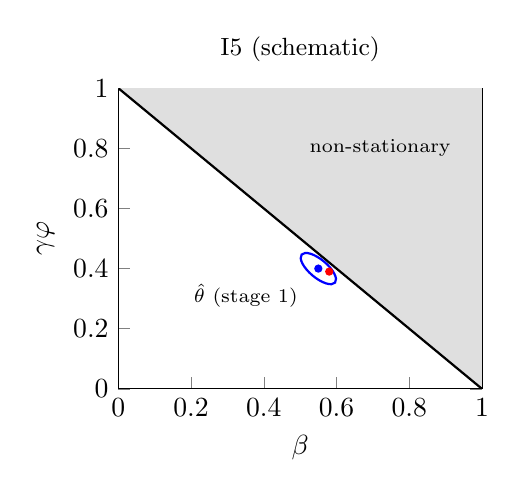
\begin{tikzpicture}
\begin{axis}[width=6.2cm,height=5.4cm,xmin=0,xmax=1,ymin=0,ymax=1,
  xlabel={$\beta$},ylabel={$\gamma\varphi$},title={I5 (schematic)},title style={font=\small}]
\addplot[name path=L,thick,domain=0:1] {1-x};
\path[name path=T] (axis cs:0,1) -- (axis cs:1,1);
\addplot[gray!25] fill between[of=L and T];
\node[font=\scriptsize] at (axis cs:0.72,0.8) {non-stationary};
\draw[blue,thick] (axis cs:0.55,0.40) ellipse [x radius=0.06,y radius=0.03,rotate=-40];
\fill[blue] (axis cs:0.55,0.40) circle (1.5pt);
\fill[red] (axis cs:0.58,0.39) circle (1.5pt);
\node[font=\scriptsize,anchor=north east] at (axis cs:0.52,0.38) {$\hat\theta$ (stage 1)};
\end{axis}
\end{tikzpicture}\hfill
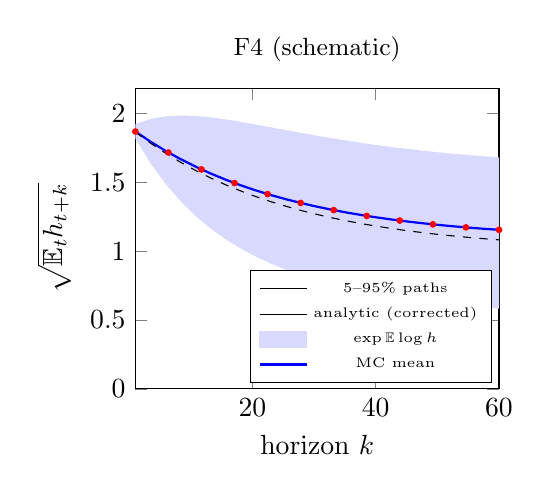
\begin{tikzpicture}
\begin{axis}[width=6.2cm,height=5.4cm,xmin=1,xmax=60,ymin=0,
  xlabel={horizon $k$},ylabel={$\sqrt{\E_t h_{t+k}}$},title={F4 (schematic)},title style={font=\small},
  legend style={font=\tiny,at={(0.98,0.02)},anchor=south east}]
\addplot[name path=hi,draw=none,domain=1:60] {1+0.9*exp(-x/25)+0.6*(1-exp(-x/10))};
\addplot[name path=lo,draw=none,domain=1:60] {1+0.9*exp(-x/25)-0.5*(1-exp(-x/10))};
\addplot[blue!15] fill between[of=hi and lo];
\addlegendentry{5--95\% paths}
\addplot[blue,thick,domain=1:60] {1+0.9*exp(-x/25)+0.08*(1-exp(-x/25))};
\addlegendentry{analytic (corrected)}
\addplot[black,dashed,domain=1:60] {1+0.9*exp(-x/25)};
\addlegendentry{$\exp\E\log h$}
\addplot[red,only marks,mark size=1pt,samples=12,domain=1:60] {1+0.9*exp(-x/25)+0.08*(1-exp(-x/25))};
\addlegendentry{MC mean}
\end{axis}
\end{tikzpicture}
\caption{Schematic sketches with illustrative numbers, not results. Left: the stationarity region with an estimate and its
confidence ellipse (I5). Right: a forecast fan in which the gap between the dashed and solid curves is the Jensen
correction (F4).}\label{fig:stat-sketch}
\end{figure}

\subsection{Forecast evaluation}\label{sec:figs-fc}
All of these use the out-of-sample protocol in Section~\ref{sec:eval}. The proxy for $h$ is $x_{t+k}$
(summed over $k$), and the loss functions are QLIKE and MSE, which are robust to proxy noise \cite{Patton2011}.
Benchmarks are GARCH(1,1) \cite{Bollerslev1986}, HAR-RV \cite{Corsi2009} and the pure (stage~1) Realized GARCH.
\begin{itemize}
\item \textbf{E1. Loss by horizon:} grouped bars or lines of mean test QLIKE and MSE against $k$, one series per
model, with block-bootstrap 95\% CIs. Report values relative to HAR (ratio $<1$ is better).
\item \textbf{E2. Diebold--Mariano path:} the cumulative loss differential $\sum_{s\le t}(L^{\rm model}_s-L^{\rm bench}_s)$
over the test dates, one line per benchmark, with the final DM statistic (HAC, \texttt{dm\_test}) in the legend
\cite{DM1995}. A steady downward slope is good. A path dominated by one or two crisis jumps is fragile.
\item \textbf{E3. Mincer--Zarnowitz regression:} a scatter of $x_{t+k}$ against $\hat h_{t+k|t}$ on log--log axes,
with the fitted line $x=a+b\hat h$ and the 45-degree line. Report $(a,b)$ with HAC s.e., the Wald test of $(0,1)$, and $R^2$ \cite{MZ1969}.
\item \textbf{E4. Model Confidence Set:} a tile chart with models as rows and horizons as columns. Shade the members of the 90\% MCS
\cite{HLN2011} and print the MCS p-value in each cell.
\item \textbf{E5. Calibration and reliability:} sort the test points into deciles of $\hat h$, then plot the mean realized $x$
against the mean $\hat h$ with the 45-degree line and CIs. A slope below 1 means forecasts are too extreme.
\item \textbf{E6. VaR backtest}, applicable only if return quantiles $\hat q_\alpha=\mu+\sqrt{\hat h}\,F^{-1}(\alpha)$ are reported.
Plot returns with the $-$VaR line and mark exceedances. Report a table of the hit rate, the Kupiec unconditional-coverage
LR \cite{Kupiec1995} and the Christoffersen independence and conditional-coverage LRs \cite{Christoffersen1998}
at $\alpha=1\%$ and $5\%$. See \cite{Tendenan2020} for Realized EGARCH tail-risk evaluation.
\end{itemize}

\subsection{Ablation study design}\label{sec:figs-abl}
Unless stated otherwise, each ablation changes one setting of the default \texttt{Config} in each of the 4 configurations.
\textbf{Protocol:} run $S\ge5$ seeds per cell, varying \texttt{cfg.seed}, which drives NN initialisation and
batch order. Stage~1 is deterministic given the data, so it is fitted once and shared. Report the mean $\pm$ s.d.\
and the 95\% $t$-interval of the test NLL ($\ell_r$ and $\ell_{rx}$ per observation) and of QLIKE at $k=1,5,22$.
Hyper-parameters are selected on validation NLL only, and the test set is touched once.
\textbf{Multiple comparisons:} about 15 ablations $\times$ 4 configurations $\times$ 3 horizons gives
roughly 180 tests, so about 9 false rejections are expected at the 5\% level. Control this with Holm or
Benjamini--Hochberg, or rely on the MCS (E4), which handles the multiplicity by construction. Seed variance and
forecast-sample variance are different sources of uncertainty, so report both.

Standard plot types:
(P1) grouped bar charts of test NLL and QLIKE with seed CIs;
(P2) a heatmap of validation NLL over the $(\lambda_m,\lambda_g)$ grid, faceted by $\lambda_{\rm orth}$;
(P3) learning curves (train loss and val NLL against epoch, as in \texttt{history}), one line per seed;
(P4) a paired DM-statistic matrix with variants on both axes and cells coloured by the HAC DM statistic;
(P5) parameter-shift plots of the stage~2 minus stage~1 change in each economic parameter, with seed CIs.

{\small
\begin{longtable}{p{3.1cm}p{4.8cm}p{2.1cm}p{4.5cm}}
\toprule
Ablation & Hypothesis & Evidence & Expected outcome\\
\midrule\endhead
NN on vs off (stage 2 vs 1) & $g$ captures structure beyond the parametric recursion & P1, P4, E2, F7 & a small NLL gain, larger in-sample than out of sample. If the test gain is not significant, report the pure model.\\
garch vs egarch & $\gamma'u_{t-1}$ with $\tau$ in the GARCH equation fits better \cite{HH2016} & P1, E1, E4, F2 & EGARCH is marginally better on the daily data.\\
daily vs 5-min & more information per day from intraday data & E1 (aggregated to daily horizons) & 5-min data improves short horizons, with parity at $k=22$.\\
$\lambda_m=0$ & the moment penalty regularises and does not just restate the likelihood & P2, R3 & a small effect, with larger moment drift when $\lambda_m=0$.\\
$\lambda_g=0$ & the $g$ penalty prevents overfitting & P2, P3, F7(b) & larger $|g|$ and a widening train/val gap.\\
$\lambda_{\rm orth}=0$ & orthogonality identifies $(\omega,\beta)$ & P5, F7(d) & $\omega$ and $\beta$ drift, and $g$ develops a slope against $\log h$.\\
no state inputs ($z_{t-1},\log h_{t-1}$) & the NN needs the state to correct the dynamics & P1, P4 & a small loss of fit, with $g$ smoother.\\
HAR features removed & long memory is what $g$ adds & P1, F7(c) & most of the stage~2 gain disappears, especially at $k=22$.\\
hidden size $\{8,32,128\}$ & capacity does not matter much & P1, P3 & a flat curve, and overfitting at 128.\\
chunk length / TBPTT $\{32,128,512\}$ & long chunks are needed for persistence & P1, P3, F7(a) & short chunks give sawtooth $g$ and worse NLL.\\
carried vs re-initialised state & re-initialising biases $h$ at chunk starts & P1, F1 & re-initialising is worse, with spikes at boundaries.\\
$\tau\equiv0$ & leverage matters & profile LR, R5, P1 & a significant LR, and nonzero $\mathrm{corr}(z_t,u_t)$.\\
no measurement equation (partial likelihood $\ell_r$) & $x$ informs $h$ only through the joint likelihood & P1 on $\ell_r$, I2 & wider s.e.\ and a worse $\ell_r$ out of sample \cite{HHS2012}.\\
\bottomrule
\end{longtable}}

\subsection{Figure-to-code checklist}\label{sec:figs-check}
{\small
\begin{longtable}{p{3.2cm}p{8.4cm}p{2.6cm}}
\toprule
Figure & Source in code & Status\\
\midrule\endhead
Training curves (P3) & \texttt{history} from \texttt{train.fit} (\texttt{train\_loss}, \texttt{val\_nll}, \texttt{stage1\_nll}, \texttt{best\_epoch}); \texttt{plot\_fit} panel 1 & exists (single seed)\\
F1 & \texttt{out["log\_h"]}, \texttt{ds.log\_x}, \texttt{ds.n\_train}, \texttt{ds.n\_val}; \texttt{plot\_fit} panel 2 & implemented (\texttt{plots.shade\_splits}, \texttt{plot\_F1})\\
F2 & \texttt{model.meas\_lev}, \texttt{params()} ($\tau_1,\tau_2$) & implemented (\texttt{plot\_F2})\\
F3 & \texttt{model.persistence}, \texttt{state\_space()} & implemented (\texttt{diagnostics.impulse\_response}, \texttt{plot\_F3})\\
F4 & \texttt{model.forecast} (analytic), \texttt{simulate\_forecast} (MC), \texttt{fc["q"]}; \texttt{plot\_fit} panel 3 & implemented (\texttt{diagnostics.forecast\_quantiles}, \texttt{plot\_F4})\\
F5 & \texttt{model.forecast} summed over $k$ & implemented (\texttt{diagnostics.term\_structure}, \texttt{plot\_F5})\\
F6 & periodicity factor in \texttt{data.py} (5-min loader) & implemented (\texttt{data.periodicity\_factor}, \texttt{df.attrs}, \texttt{plot\_F6})\\
F7 & \texttt{out["g"]}/\texttt{correction()}, \texttt{out["g\_next"]} & implemented (\texttt{diagnostics.partial\_dependence}, \texttt{plot\_F7})\\
R1, R2, R5 & \texttt{out["z"]}, \texttt{out["u"]}, \texttt{model.sigma\_u} & implemented (\texttt{diagnostics.residual\_stats}, \texttt{ljung\_box}, \texttt{plot\_R1}, \texttt{plot\_R2}, \texttt{plot\_R5})\\
R3 & \texttt{losses.moment\_residuals} (scalar only) & implemented (\texttt{diagnostics.moment\_paths}, \texttt{plot\_R3})\\
R4 & \texttt{out["z"]} & implemented (\texttt{plot\_R4})\\
I1, I2 & \texttt{train.stage1\_qmle}, \texttt{nll\_parts} (per-obs scores via autograd) & implemented (\texttt{diagnostics.profile\_likelihood}, \texttt{standard\_errors}, \texttt{plot\_I1}, \texttt{plot\_I2})\\
I3 & \texttt{model.simulate}, \texttt{load\_params} & implemented, off by default (\texttt{diagnostics.parameter\_recovery}, \texttt{plot\_I3})\\
I4 & a loop over \texttt{stage1\_qmle} & implemented, off by default (\texttt{diagnostics.rolling\_params}, \texttt{plot\_I4})\\
I5 & \texttt{params()}, \texttt{pinn\_persistence}; \texttt{evaluate()["garch11"]} & implemented (\texttt{diagnostics.stationarity\_point}, \texttt{plot\_I5})\\
E1 & \texttt{evaluate()["k=<k>"][name]["qlike"/"mse"]}; \texttt{plot\_fit} panel 4 & partial (QLIKE only, no CIs)\\
E2 & \texttt{evaluate.dm\_test}, \texttt{["k=<k>"]["dm"]} (statistic only) & implemented (\texttt{evaluate(return\_series=True)}, \texttt{diagnostics.cumulative\_loss\_diff}, \texttt{plot\_E2})\\
E3, E5 & per-$t$ forecasts from \texttt{\_model\_sum\_forecasts} & implemented (\texttt{diagnostics.mincer\_zarnowitz}, \texttt{calibration\_deciles}, \texttt{plot\_E3}, \texttt{plot\_E5})\\
E4 & none & implemented, approximate (\texttt{diagnostics.model\_confidence\_set}, \texttt{plot\_E4})\\
E6 & none (return quantiles not produced) & implemented (\texttt{diagnostics.var\_backtest}, \texttt{kupiec}, \texttt{christoffersen}, \texttt{plot\_E6})\\
Test NLL & \texttt{evaluate()["loglik"]} (\texttt{l\_r}, \texttt{l\_rx}) & exists\\
Ablation plots P1, P2, P4, P5 & multi-run driver over \texttt{Config} (\texttt{use\_nn}, \texttt{nn\_state\_inputs}, \texttt{lambda\_*}, \texttt{hidden\_dim}, \texttt{chunk\_len}) & TODO\\
\bottomrule
\end{longtable}}

%======================================================================
\section{Implementation mapping}
%======================================================================
\paragraph{\texttt{data\_utils.py}.} Currently computes a 5-minute log-return series and a
78-bar rolling sample variance $\times19656$, then trains on the 5-minute series. It should:
(i) after the GMT/BST timestamp adjustment, group bars by trading day and session;
(ii) compute per day $RV_t=\sum_j r_{t,j}^2$ (\% units, \eqref{eq:rv}) using only within-session
returns, $r^{oc}_t$, $r^{on}_t$, $r^{cc}_t$ (\eqref{eq:oc}--\eqref{eq:cc}); drop days with too
few bars or $RV_t=0$; (iii) return one row per day $(r_t,x_t)$ and the HAR features;
(iv) split chronologically (train/val/test); no overlapping 20-step windows and no shuffling.
Remove the annualisation factor from model inputs.

\paragraph{\texttt{models.py}.} A \texttt{RealizedGARCH} module with raw parameters as in
Section~\ref{sec:param}; one leverage function $\tau$ used only in the measurement
equation; a \texttt{filter(r, x, h1)} method implementing Algorithm~\ref{alg:filter} with
observed $\log x_{t-1}$ in the GARCH equation, returning $\log h$, $z$, $u$, $\ell_r$, $\ell_x$;
a \texttt{neg\_loglik} method returning $-\ell(r,x)/n$ \eqref{eq:ll-joint}; an optional
\texttt{RealizedGARCHPINN} subclass adding $s\,g_\eta(\mathbf f_{t-1})$ with lagged inputs only,
no BatchNorm, no clamps, no \texttt{0.005} hard scale; a \texttt{moment\_residuals} method for
\eqref{eq:moments}. Delete \texttt{return\_loss}, \texttt{garch\_loss}, \texttt{data\_loss},
\texttt{smoothness\_penalty}; drop the 78-bar \texttt{generate\_time\_features}
(daily calendar features may be passed in from the data instead). A separate
\texttt{RealizedEGARCH} class, if wanted, implements
\eqref{eq:reg-garch}--\eqref{eq:reg-meas}.

\paragraph{\texttt{training.py}.} \texttt{train\_model}: Algorithm~\ref{alg:train}
(Stage-1 L-BFGS QMLE, Stage-2 Adam on \eqref{eq:pinn-loss}, early stopping on validation
likelihood); no anomaly detection in production. \texttt{forecast\_volatility}:
Algorithm~\ref{alg:fc}, starting from $\log h_{t+1}$ computed with the observed $x_t$, iterating
with $\pi$ and $\mu_h$, dropping $\tau$ via $\E\tau(z)=0$, and returning both
$\E_t h_{t+k}$ and $\E_t x_{t+k}$ with the corrections \eqref{eq:fc-h}, \eqref{eq:fc-x}.
Add an \texttt{evaluate} function for QLIKE/MSE \eqref{eq:mse}--\eqref{eq:qlike} and a HAR-RV
benchmark \eqref{eq:har}, and a simulation test (Algorithm~\ref{alg:sim}).

\begin{thebibliography}{99}
\bibitem{ABDL2003} T.~G. Andersen, T.~Bollerslev, F.~X. Diebold, P.~Labys (2003).
Modeling and forecasting realized volatility. \emph{Econometrica} 71(2), 579--625. (NBER WP 8160.)
\bibitem{AB1997} T.~G. Andersen, T.~Bollerslev (1997). Intraday periodicity and volatility
persistence in financial markets. \emph{Journal of Empirical Finance} 4, 115--158. (NBER WP 5752.)
\bibitem{BNS2002} O.~E. Barndorff-Nielsen, N.~Shephard (2002). Econometric analysis of
realised volatility and its use in estimating stochastic volatility models. \emph{JRSS B}
64(2), 253--280. (Nuffield WP 2001-W4.)
\bibitem{Bollerslev1986} T.~Bollerslev (1986). Generalized autoregressive conditional
heteroskedasticity. \emph{Journal of Econometrics} 31, 307--327.
\bibitem{Corsi2009} F.~Corsi (2009). A simple approximate long-memory model of realized
volatility. \emph{Journal of Financial Econometrics} 7(2), 174--196.
\bibitem{HH2016} P.~R. Hansen, Z.~Huang (2016). Exponential GARCH modeling with realized
measures of volatility. \emph{Journal of Business \& Economic Statistics} 34(2), 269--287.
\bibitem{HHS2012} P.~R. Hansen, Z.~Huang, H.~H. Shek (2012). Realized GARCH: a joint model for
returns and realized measures of volatility. \emph{Journal of Applied Econometrics} 27(6),
877--906. (CREATES RP 2010-13.)
\bibitem{Liu2023} C.~Liu, C.~Wang, M.-N. Tran, R.~Kohn (2023). Deep learning enhanced
realized GARCH. arXiv:2302.08002.
\bibitem{Nelson1991} D.~B. Nelson (1991). Conditional heteroskedasticity in asset returns: a
new approach. \emph{Econometrica} 59(2), 347--370. (Not obtained.)
\bibitem{Patton2011} A.~J. Patton (2011). Volatility forecast comparison using imperfect
volatility proxies. \emph{Journal of Econometrics} 160(1), 246--256. (Working paper, Dec.\ 2008.)
\bibitem{Raissi2019} M.~Raissi, P.~Perdikaris, G.~E. Karniadakis (2019). Physics-informed
neural networks. \emph{Journal of Computational Physics} 378, 686--707. (arXiv:1711.10561, Part I.)
\bibitem{Tendenan2020} V.~Tendenan, R.~Gerlach, C.~Wang (2020). Tail risk forecasting using
Bayesian realized EGARCH models. arXiv:2008.05147.
\bibitem{Xu2024} Z.~Xu, J.~Liechty, et al.\ (2024). GARCH-informed neural networks for
volatility prediction in financial markets. arXiv:2410.00288.
\bibitem{Zhao2024} P.~Zhao, H.~Zhu, W.~S.~H. Ng, D.~L. Lee (2024). From GARCH to neural
network for volatility forecast. arXiv:2402.06642.
\bibitem{Christoffersen1998} P.~F. Christoffersen (1998). Evaluating interval forecasts. \emph{International Economic Review} 39(4), 841--862. (Not in \texttt{papers/}.)
\bibitem{DM1995} F.~X. Diebold, R.~S. Mariano (1995). Comparing predictive accuracy. \emph{J. Business \& Economic Statistics} 13(3), 253--263. (Not in \texttt{papers/}.)
\bibitem{HLN2011} P.~R. Hansen, A.~Lunde, J.~M. Nason (2011). The model confidence set. \emph{Econometrica} 79(2), 453--497. (Not in \texttt{papers/}.)
\bibitem{Kupiec1995} P.~H. Kupiec (1995). Techniques for verifying the accuracy of risk measurement models. \emph{J. Derivatives} 3(2), 73--84. (Not in \texttt{papers/}.)
\bibitem{MZ1969} J.~Mincer, V.~Zarnowitz (1969). The evaluation of economic forecasts. In \emph{Economic Forecasts and Expectations}, NBER, 3--46. (Not in \texttt{papers/}.)
\end{thebibliography}

\paragraph{Note on ``physics-informed''.} In \cite{Raissi2019} the physics is a differential
equation whose residual is evaluated at collocation points and added to the data loss. The
analogue here is the Realized GARCH system; because the filter \emph{solves} the GARCH and
return equations exactly, their residuals vanish by construction, and the information
content of the model is carried by the likelihood \eqref{eq:ll-joint} and the moment
conditions \eqref{eq:moments}, not by residual MSEs \derived.

\end{document}
